\PassOptionsToPackage{square}{natbib}
\documentclass{article}

% if you need to pass options to natbib, use, e.g.:
% \PassOptionsToPackage{numbers, compress}{natbib}
% before loading nips_2016
%
% to avoid loading the natbib package, add option nonatbib:

\usepackage[final]{nips_2016} % produce camera-ready copy

% to compile a camera-ready version, add the [final] option, e.g.:
% \usepackage[final]{nips_2016}

\usepackage[utf8]{inputenc} % allow utf-8 input
\usepackage[T1]{fontenc}    % use 8-bit T1 fonts
\usepackage{hyperref}       % hyperlinks
\usepackage{url}            % simple URL typesetting
\usepackage{booktabs}       % professional-quality tables
\usepackage{amsfonts}       % blackboard math symbols
\usepackage{nicefrac}       % compact symbols for 1/2, etc.
\usepackage{microtype}      % microtypography
\usepackage{graphicx}

\title{Musical Instruments Recognition based on Convolutional Neural Networks}

% The \author macro works with any number of authors. There are two
% commands used to separate the names and addresses of multiple
% authors: \And and \AND.
%
% Using \And between authors leaves it to LaTeX to determine where to
% break the lines. Using \AND forces a line break at that point. So,
% if LaTeX puts 3 of 4 authors names on the first line, and the last
% on the second line, try using \AND instead of \And before the third
% author name.

\author{
  Ci Li\\
  \texttt{cil@kth.se} \\
  %% examples of more authors
  \And
  Mengdi Xue \\
  \texttt{mengdix@kth.se} \\
}

\begin{document}
% \nipsfinalcopy is no longer used

\maketitle

\begin{abstract}
  In this project, we use Convolutional Neural Networks (CNNs) and try different parameter settings to build and train a model for music instruments recognition. We build a base model which consists of two convolutional layers, two max pooling layers, and a fully connected layer. We use the NSynth dataset, which is developed by Google containing high-quality musical notes. We then experiment on different parameter settings and finally test the model on real music. As for evaluation, we use accuracy, cross-entropy loss and confusion matrices to measure the performance of our model. 
\end{abstract}

\section{Introduction}

Recently, with the development of digital music creation, there are a large amount of music audio data collected and restored by many organizations. Thus, it is very important to figure out methods to make use of these music data and help people to retrieve the digital audio signal and analyze the content of audio data. Music instrument recognition is one part of these. It is one aspects of audio content analysis, which has a lot of approaches, such as singer recognition, audio information extracting, audio coding, etc. Also, it has a lot of applications, for example, it can be used in content-based music transcription, structured music coding, and music recommending and query engines, etc. So in this project we want to recognize different music instruments due to the above reasons. In previous research on music instrument recognition, models like logistic regression, K-NN, SVM \cite{sell}, Naive Bayes model, multilayer perceptron (MLP), Radial Basis Functions (RBFs) \cite{deng}, quadratic discriminant analysis \cite{agostini}, etc. are applied. As for feature extracting, Mel-frequency cepstral coefficients (MFCC) features, linear prediction cepstral and delta cepstral coefficients are commonly used in musical instrument recognition . But MFCC performs better in music instrument recognition according to \cite{eronen}. In our project, we tried another model based on MFCC feature.

Deep Neural Networks (DNNs) is one of the machine learning tools based on multi-layer feed-forward artificial neural networks. It is designed to imitate human brain structure and is used to recognize patterns. Convolutional Neural Networks (CNNs) is one variant of DNNs, which is also a kind of feed-forward artificial neural networks. They are now successfully applied to many scientific fields and become a new trend because CNNs avoid the complex pre-processing of the image, and people can use the original image as the input directly. CNNs are also known as shift invariant or space invariant artificial neural networks (SIANN), based on their shared-weights architecture and translation invariance characteristics.\cite{zhang} As a result, people use CNNs to convolute the image, audio or video image and try to recognize features based on convolutional parts of the images. They have outstanding performances in image and video recognition \cite{krizhevsky} and successful applications in music recommending systems \cite{vanden} and automatic speech recognition (ASR) systems \cite{abdelhamid}. CNNs have also been successfully applied to musical instrument recognition in real-world polyphonic music \cite{yoonchang}. But it also has limits that it needs a large amount of computational resources to run, which has not yet been solved.

Since CNNs has been successfully applied to image recognition systems, ASR systems and even musical instruments recognition systems, in our project, we applied CNNs architecture on MFCC feature of the audio data of different instruments with variant notes and tried to classify their music instruments family. The goal of our project is to build models to recognize music instrument with CNNs, try different parameter settings to see their performances and apply the model on real data. We will use the same CNNs architecture to train our model and evaluate how they perform based on their accuracy, loss and confusion matrices. In Section 2, we describes our CNNs architecture and data representation. Next, we show details of our experiments in Section 3 and the performances of the experiments in Section 4. Finally, Section 5 contains our discussions and conclusions based on our experiments.

% 最后介绍一下其他的section

\section{Method}

\subsection{Model Architecture}

As mentioned earlier, CNNs are successfully applied to ASR and image recognition fields. That is because, in the image and speech domain, using traditional neural networks will consume too much computational resources. Usually, the size of MFCC feature of an utterance is a two-dimension matrix that has length of the time length (assume it's t here) and width of 13 according to MFCC feature extraction. If a traditional fully connected network structure is used, which means the nerves in the network will be connected to each neuron on the adjacent layer, then the network will have 13*t neurons. Assume we have m hidden nodes and have output size of n, then we need weight parameter size of 13*t*m*n, which will be too large if we have long time sequences and more classes to recognize. However, CNNs will solve this problem.

In this project, we applied a typical CNNs architecture on our MFCC features. It is composed of two convolutional layers, two max pooling layers, one fully connected layer with softmax, as in Figure \ref{fig:cnn}. We will introduce them in detail in the following.

\begin{figure}[h!]
\centering
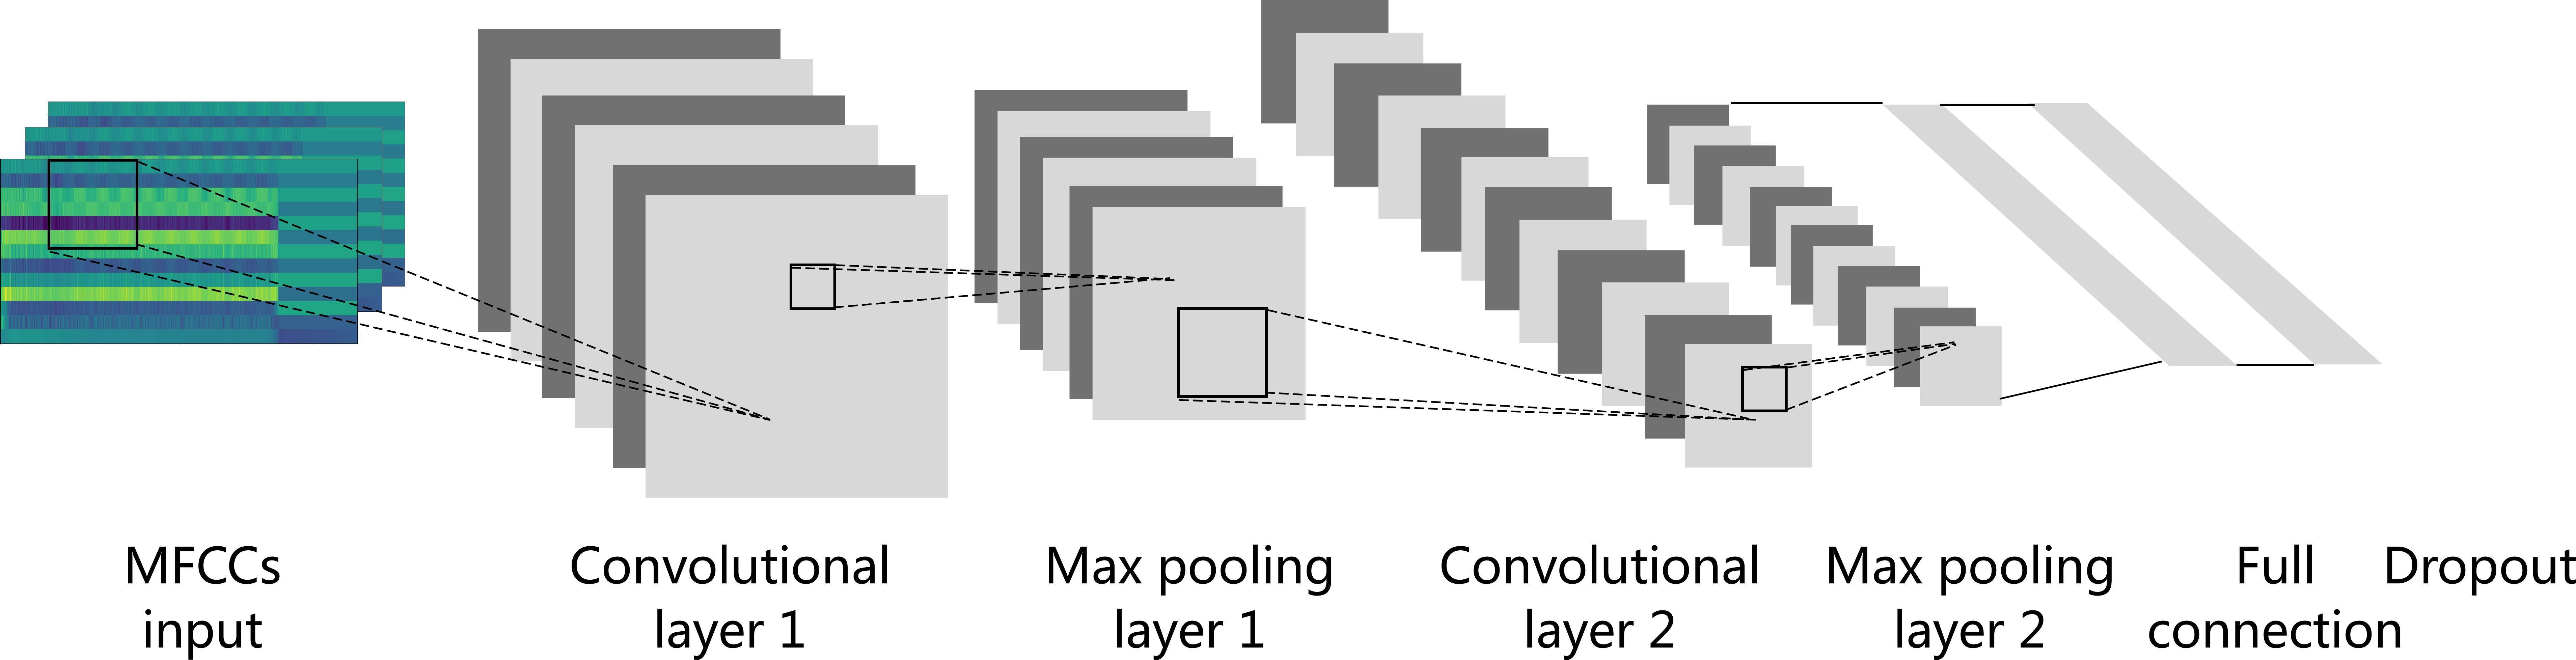
\includegraphics[width=\textwidth]{cnnarchitecture.png}
\caption{CNNs architecture overview}
\label{fig:cnn}
\end{figure}

Firstly, the convolutional layer is accomplished by applying a number of filters, which is also called kernels, to the input matrix. It convolves the input matrix with each filter, slides the filter over all spatial locations in image and outputs one number each time, which is the dot product between the filter and the convolved input matrix that has the same size of the filter. Then, the features are correlated in each output and the outputs will be stacked together. This means the convolutional kernels can extract, or detect specific features of the original input and stacking all they learned together to get a global result. Usually, we use the first convolutional layer to find basic features and apply the second convolutional layer to find some relatively complex features based ont he basic features. Bigger size of convolutional kernels will embody more detailed features of the input. In our architecture, the two convolutional layers both have filter size of 5 by 5. The first layer has 32 filters and the second layer has 64 filters.

Then, after each convolutional layer, a pooling layer is applied to each window to return a more independent value of each filter as the output. The commonly used pooling methods are finding the maximum value, average, or median value. The goal of pooling is to extract the independent features that are more representative so that after subsequent calculations, the size of the feature map, the size of parameters, and the amount of calculation are reduced, but the effect is not lost. In our architecture, we applied max pooling as usual to extract the largest value of the window to represent each window.

After the second max pooling layer, usually, a fully connected layer with softmax will be used to classify. The output of the second max pooling layer will be flattened to vectors and used as input of the fully connected layer. In our architecture, we applied one fully connected layer with softmax and add a dropout layer to improve the generalization of the network.

To evaluate the network, a cross entropy loss was applied to calculate the loss of training set and validation set. In neural networks, cross entropy function is usually used with softmax classifier. Softmax classifier calculates the probability vector the network assigns to the input for each class, and cross entropy loss computes the negative log-likelihood of the training data, as in Equation \ref{con:crossentropy}.

\begin{equation}
L(D, W, b)=-\frac{1}{|D|}\sum_{(x,y)\in D}log(\frac{exp(s_y)}{\sum_{k=1}^{C} exp(s_k)}) \label{con:crossentropy}  
\end{equation}

As for the gradient optimization, Adam optimizer is applied in our architecture. It is a method for efficient stochastic optimization that only requires first-order gradients with little memory requirement.\cite{adam} It is based on stochastic gradient descent, which is more efficient, more suitable for solving optimization problems with large scale data and parameters, more suitable for solving problems with high noise or sparse gradients, and needs less adjustments of parameters.

\subsection{Data Representation}

\subsubsection{The NSynth Dataset}

The NSynth\cite{nsynth} is an audio database released by Google containing high-quality musical notes. The NSynth has 1006 standard instruments with totally 11 instrument families including Bass, Brass, Flute, Guitar, Keyboard, Mallet, Organ, Reed, String, Synth Lead, and Vocal. Each family includes different audio samples with different velocities ranging over different pitch of a standard MIDI piano. Each audio file contains four seconds audio of the corresponding instrument with multiple features in note. The NSynth provides data in two formats: one is tfrecord, which can be directly used in Tensorflow, and another is raw audios in format of wav files. There are totally 289,205 samples in training set, 12,678 samples in validation set and 4,096 samples in testing set. 

\subsubsection{Feature Extraction}

Mel-frequency cepstral coefficients (MFCCs) are coefficients that collectively make up an Mel-frequency cepstral (MFC) which is a representation of the short-term power spectrum of a sound.\cite{mfcc} MFCCs is one of the audio features usually used in Speech Technology and music genre classification. 

\begin{figure}[h!]
\centering
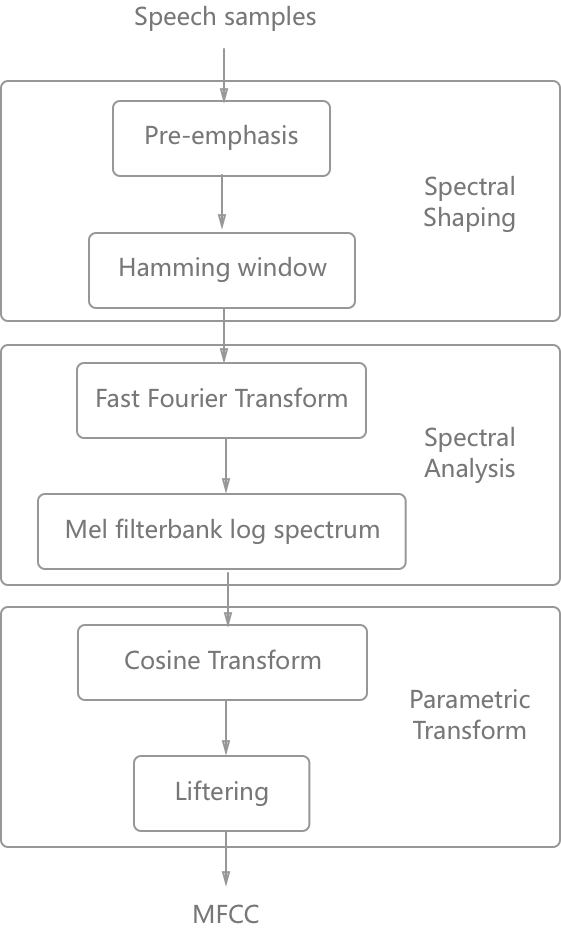
\includegraphics[width=0.3\textwidth]{mfcc-process.png}
\caption{MFCC process}
\label{fig:mfcc}
\end{figure}

MFCCs is generated by 6 steps shown in Figure \ref{fig:mfcc}. Firstly, it enframes the input to extract frames of samples over time from the input speech sample. Next, the pre-emphasis step is a high frequency filter to emphasize the energy of high frequency which is suppressed by the pronunciation system in each frame. Next step of spectral shaping is to apply hamming window to the frames of speech signal in order to smooth the values and reduce spectral leakage. Then, it comes to spectral analysis part. Fast Fourier transform(FFT) converts the signal in time domain to energy distribution in the frequency domain. Different energy distribution can represent different characteristics of different voice. However, human ear is sensitive to different frequency bands. So the Mel filterbank log spectrum can help the signal fit the property of non-linear human ear perception of sound. The last part is parametric transform. After discrete cosine transform(DCT), the energy will focus on the media and the low frequency part, so it is common to use the top 13 coefficients as the result of DCT. Finally liftering function is used to correct the range of the coefficients.


% 来一段mfcc的介绍科科。\\ 
% 哇通过分段,预加重,加窗,傅立叶变换,三角滤波,DCT。经过DCT之后,中低频的数据包含大部分信息,所以只取了前13维作为数据,再过一个lifter,生成极具特色的mfcc。\\

\section{Experiments}

In this section, we will present our result of the experiments using tensorflow to build CNNs on the MFCCs features of the NSynth dataset. We will also provide results of some variations of the model in section 2 to try to analyze the influences of different parameters.

\subsection{Data Pre-processing}

The overall data processing is as following. We read the sampling rate, musical instrument family and audio data from the tfrecord file of each dataset. Then we calculated the lifted MFCCs of each utterance using their audio data and sampling rate and stored them with their target instrument family. So we have 289,205 samples in training set, 12,678 samples in validation set, and 4,096 samples in testing set.

The training dataset has 289,205 samples in total but the data for each classes are unbalanced as shown in Table \ref{tab:dataset}. It is known that machine learning classifiers may fail to deal with imbalanced training datasets because they are sensitive to portions of different classes. So we pre-processed the training set in order to have balanced data for training. In order to achieve this, we randomly sampled 10,000 utterances with replacement from each class for training and shuffled the examples for the network to convergence faster. Eventually, we have 110,000 training data in total. Also, we normalised over the whole training set, calculated the means and covariances and stored them to normalise the validation set and testing set when using them.

\begin{table}[t]
  \caption{NSynth: size of each class in every dataset}
  \label{tab:dataset}
  \centering
  \begin{tabular}{llllllllllll}
    \toprule
    Dataset  &Bass	& Brass	& Flute	& Guitar	& Keyboard	& Mallet\\
    \midrule
    train & 62836	& 11789	& 8303	& 30609	& 49417	& 33538\\
    test & 2638	& 886	& 470	& 2081	& 2404	& 663\\
    valid & 3481	& 1155	& 650	& 2733	& 3170	& 865\\
    total & 68955	& 13830	& 9423	& 35423	& 54991	& 35066\\
    \toprule
    Dataset  & Organ & Reed	& String    & Synth	& Vocal\\
    \midrule
    train	& 32879	& 13191	& 18660	& 5501	& 9804\\
    test   & 1598	& 720	& 814	& 0	    & 404\\
    valid    & 2100	& 955	& 1120	& 0	    & 545\\
    total   & 36577	& 14866	& 20594	& 5501	& 10753\\
    \bottomrule
  \end{tabular}
\end{table}

\subsection{Experimental Setup}

In our experiments, we used Tensorflow to build our CNNs architecture for training. Tensorflow is a deep learning framework provided by Google, which supports multiple platforms. It can run both on CPUs and GPUs and provides rich libaries for different algorithms, architectures and frameworks. As a result, we used it to build CNNs and run our model on GPUs. CNNs need a lot of computations based on matrices and convolutions, so GPUs can help CNNs to compute much faster than CPUs.

Our MFCCs record has size of 299 by 13. The basic settings we used is the typical 32 kernels for the first convolutional layer and 64 kernels for the second convolutional layer, which are all of size 5 by 5. And we used two max pooling layer of size 2 by 2 after each convolutional layer. So the output of our convolutional part is 73 by 2. Then we used mini-batch training with Adam algorithms to train. As for evaluating, we calculated the cross entropy loss for both training set and validation set. We only sampled 400 samples from validation set each time to save calculation time because the validation set is too large here. Eventually, we calculated and output the final accuracy and loss of the training set, the validation set and the testing set.

\subsection{Experimental Parameters}

Since we used CNNs in our experiments, the main parameters for setting is the filter size, batch size, step size, learning rate, and number of epoches.

In the following section, we will present the results based on different batch size and filter size. However, for other parameters, we have the following settings as default settings:

\small
\setlength{\parindent}{5ex}
$batch\_size = 400$\par
\setlength{\parindent}{5ex}
$learning\_rate = 1e-4$\par
\setlength{\parindent}{5ex}
$training\_epochs = 20$\par
\setlength{\parindent}{5ex}
$steps = train\_data\_size/batch\_size$\par

\section{Results}

\subsection{Base Result}

Our basic architecture has the same parpameters as described in 3.3. Then we computed their loss trends and accuracy trends of the training set and the validation set during training. The shadow orange line is the original loss calculated based on each training batch and the orange line is the smoothed trend of the training loss. Similarly, the shadow blue line is the original loss calculated on 400 sampled validation data and the blue line is the smoothed trend of the validation loss. The result is as in Figure \ref{fig:accuracy_loss_400}. It can be seen that the trend of the validation loss is decreasing so the model does not overfit. The result accuracy of the whole training set is 92.89\%, accuracy of the whole validation set is 34.44\% and the accuracy on testing set is 34.02\%.

\begin{figure}[h!]
\centering
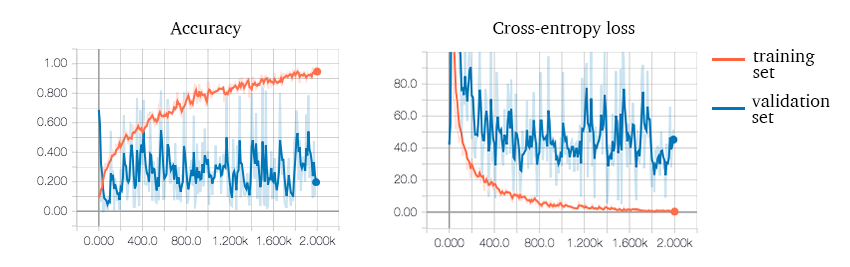
\includegraphics[width=\textwidth]{accuracy_loss_400.png}
\caption{Accuracy and loss of the training set and the validation set}
\label{fig:accuracy_loss_400}
\end{figure}

\subsection{Results of different batch size}

Then we changed the batch size smaller to 200 and use the same settings for other parameters. The result accuracy and loss is as in Figure \ref{fig:accuracy_loss_200}. The result accuracy of this model on training set is 97.07\%, on validation set is 37.37\% and on testing set is 37.20\%. We can see that the behavior of this model is better than the model using batch size of 400. Also, the trend of the loss of training and validation on this model decreases much faster than the previous model.

\begin{figure}[h!]
\centering
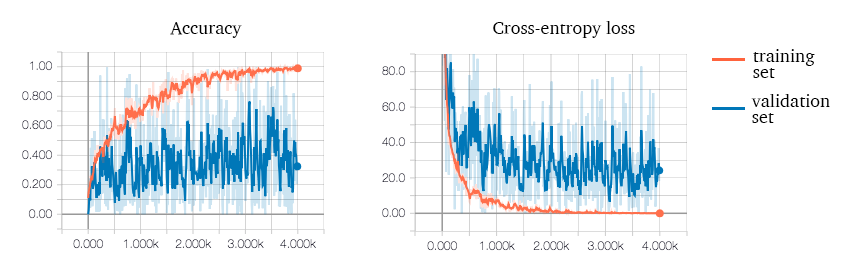
\includegraphics[width=\textwidth]{accuracy_loss_200.png}
\caption{Accuracy and loss of the training set and the validation set}
\label{fig:accuracy_loss_200}
\end{figure}

\subsection{Results of training with three subsets}

When we extracted the dataset, we separated them into 3 subsets for easier storing. So we tried to fit the model on the subsets one by one and store the model when the training of each subset is done for the next subset to train. Here we use batch size of 200. The accuracy and loss of this model is as in Figure \ref{fig:accuracy_loss_200_apart}. We can see that the accuracy and loss have a stepped form. Every time when we use the old model and a new subset to train, the accuracy on the training set goes down a little and correspondingly, the loss increases a little. But the overall trend of validation set is better than the above 2 models.

\noindent Based on this model, we get accuracy on training set of 97.23\%, on validation set of 45.81\% and on testing set of 44.87\%. The accuracy after each subsets is as in Table \ref{tab:accuracy_loss_200_apart}.

\begin{figure}[h!]
\centering
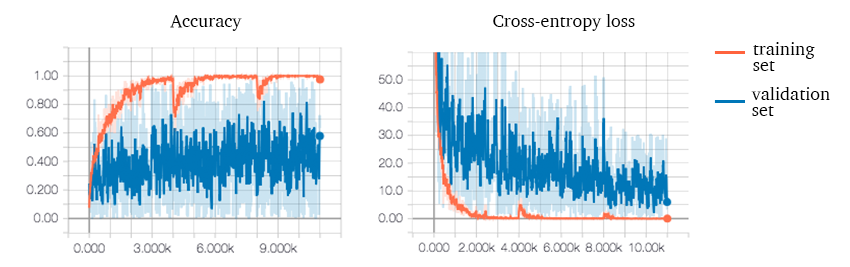
\includegraphics[width=\textwidth]{accuracy_loss_200_apart.png}
\caption{Accuracy and loss of the training set and the validation set}
\label{fig:accuracy_loss_200_apart}
\end{figure}

\begin{table}[t]
  \caption{Accuracy after training of each subsets}
  \label{tab:accuracy_loss_200_apart}
  \centering
  \begin{tabular}{llll}
    \toprule
    Subset  &Training	& Validation	& Test\\
    \midrule
    1 & 95.89\%	& 38.09\%	& 38.05\%\\
    2 & 97.91\%	& 42.54\%	& 41.80\%\\
    3 & 97.23\%	& 45.81\%	& 44.87\%\\
    \bottomrule
  \end{tabular}
\end{table}

\subsection{Confusion matrix}

We also computed the confusion matrices of the predictions using the testing set. The result is as in Figure \ref{fig:confusionmatrix}. We randomly sampled 400 records with replacement from testing set and calculated the predictions using the basic model. Then we used the predictions to compute the confusion matrices. In the figure, lighter nodes means more gathered predictions. We can see from the figure that it performs a diagonal line which means that most of the predictions corresponding to each class are right. Since there is no data for class 9 in validation set and testing set, which we can see from Table \ref{tab:dataset} before, there's no prediction corresponding to class 9.

\begin{figure}[h!]
\centering
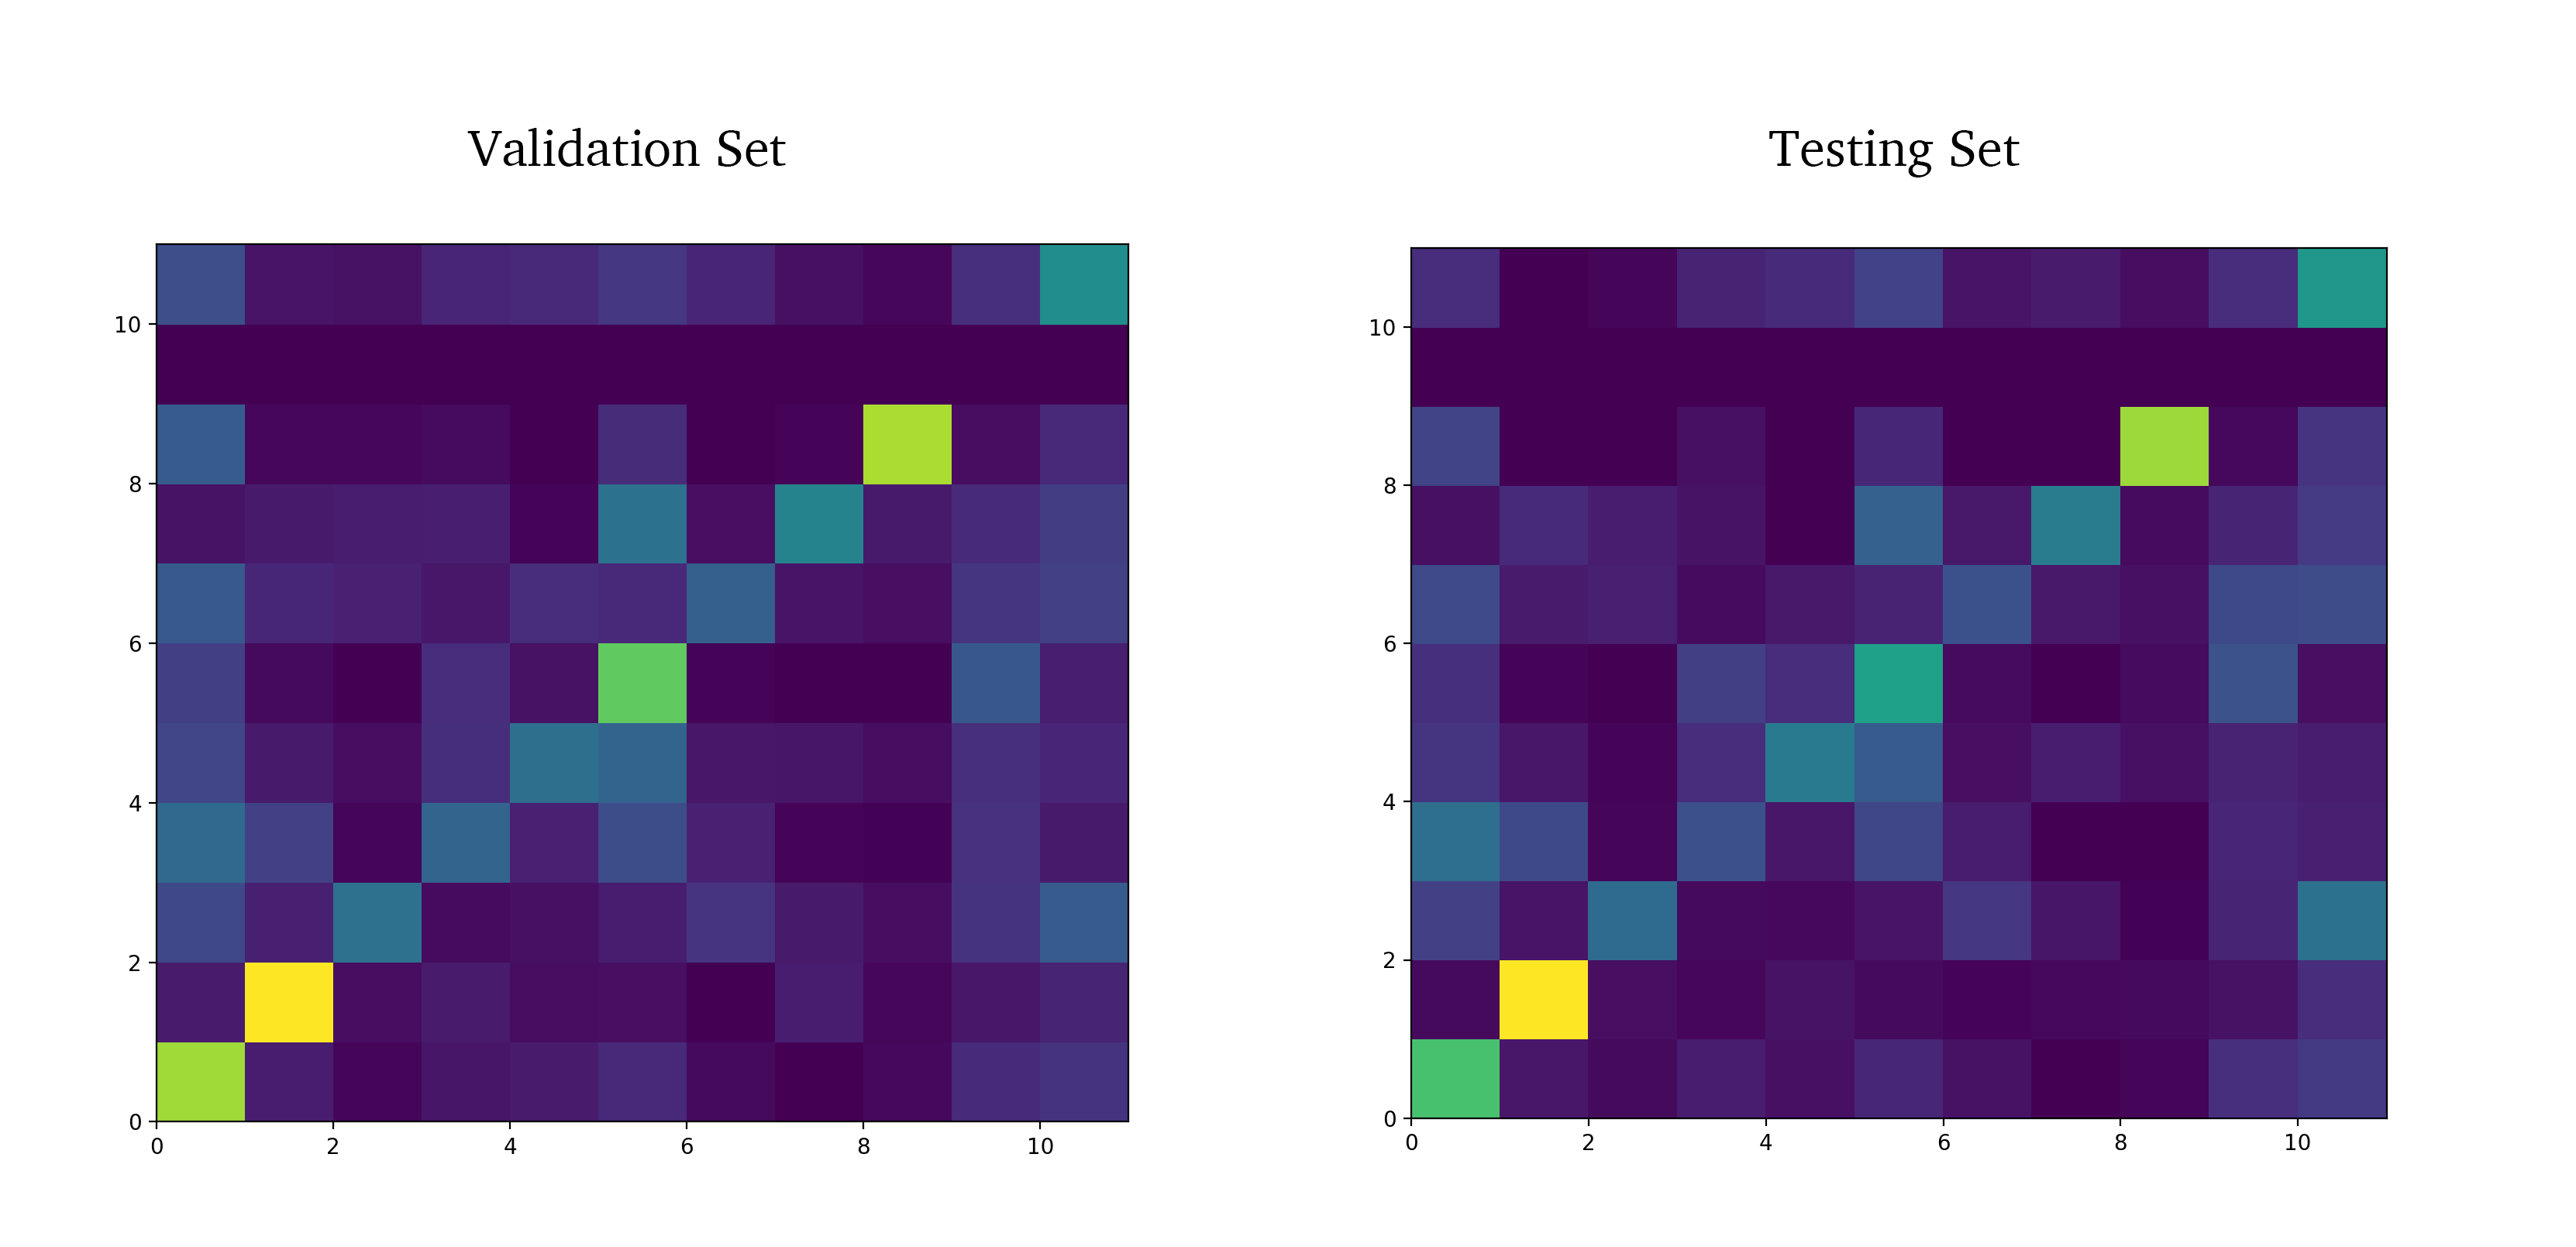
\includegraphics[width=0.8\textwidth]{confusionmatrix.png}
\caption{Confusion matrix of results on validation and testing sets}
\label{fig:confusionmatrix}
\end{figure}

\noindent The instrument family name corresponds to their representing number is as in Table \ref{tab:confusionmatrix}. We can see from the confusion matrix that family of 0, 1, 5, and 8, corresponding to Bass, Brass, Mallet, and String, are the classes that have higher classification accuracy.

\begin{table}[t]
  \caption{Instrument family names}
  \label{tab:confusionmatrix}
  \centering
  \begin{tabular}{llllllllllll}
    \toprule
    Number  &0 &1 &2 &3 &4 &5\\
    \midrule
    Family name &Bass & Brass & Flute & Guitar & Keyboard &Mallet\\
    \toprule
    Number  &6 &7 &8 &9 &10\\
    \midrule
    Family name &Organ & Reed	& String    & Synth	& Vocal\\
    \bottomrule
  \end{tabular}
\end{table}

\subsection{Play with real world music}

\noindent In order to test our model with real world music, we choose two different music files for testing. One is pure piano music and one is a mixture of orchestra instruments. After playing with the music, we have got some practical result and do some analysis.

\noindent First, we should consider the stride of the sliding window. We calculate the average time cost for one mfcc features that the CNN need to process. It is about 0.007 secs to generate one prediction in our network and the stride should not be larger than this value.

\noindent When we test the model with pure piano music, it should always output "keyboard" prediction if it works well, however, it doesn't. When we use a sliding window with 4 second and feed the transformed mfcc data to the network, it gives us predictions randomly. We address the problem on the NSynth dataset. The last one second of our training data are mostly silent. So when we test with pure piano music, we change the size of sliding window to 3 seconds and add 1 second with zeros. In this time, "keyboard" always occurs in the top 3 prediction. But the network still gives "bass" prediction with high probability. We guess the problem is that the training data has too much low frequency component and the bass also has low frequency among all instruments. For mixture music, the network has bad performance (only produce random prediction).

\noindent In order to solve the problems mentioned above, we should filter the Nsynth data and only use the first 3 second data for training. And if we want to give the network with ability to handle mixture music, we have to make fusion of training data (and multi-label for each data sample). We will do these experiments in the future.

\section{Discussion and Conclusions}

From the results of our experiments, we found that a relatively smaller batch size performs better. When batch size is bigger, more data will be given to the network to fit in each iteration. They can both converge to a relative small loss but large-batch methods tend to converge to sharp minimizers of the training and testing functions, and sharp minima lead to poorer generalization \cite{keskar}. Due to time limitation, we didn't try more batch sizes, but if time allows, it's better to try different batch sizes and choose the most suitable one.

\noindent Moreover, we didn't expect that training the three subsets to perform better than training a whole training set together. But we think one reason behind it is that the training process performs much more iterations than training a whole training set with 20 epoches, as we can see from Figure \ref{fig:accuracy_loss_200} and Figure \ref{fig:accuracy_loss_200_apart} that the former only has 2000 iterations but the latter has 12000 iterations.

\noindent In the future, we plan to do some more experiments, such as trying more different parameter settings and tuning the networks to improve its performance. Also, we plan to filter the Nsynth dataset for improving performance and add fusion data in order to give model ability of handling mixture music.

\noindent Finally, we conclude that CNNs are good models for music instruments recognition and we hope to discover more on this topic in the future.

% TODO:

% 1.DATA NORMALISZATION

% 2.conv filter

% 3.add one more fc layer


\begin{thebibliography}{9}

\bibitem{sell}
Sell, Greg, Gautham J. Mysore, and Song Hui Chon. "Musical Instrument Detection." \textit{Center for Computer Research in Music and Acoustics} (2006).

\bibitem{deng}
Deng, Jeremiah D., Christian Simmermacher, and Stephen Cranefield. "A study on feature analysis for musical instrument classification." \textit{IEEE Transactions on Systems, Man, and Cybernetics, Part B (Cybernetics)} 38.2 (2008): 429-438.

\bibitem{agostini}
Agostini, Giulio, Maurizio Longari, and Emanuele Pollastri. "Musical instrument timbres classification with spectral features." \textit{EURASIP Journal on Advances in Signal Processing} 2003.1 (2003): 943279.

\bibitem{eronen}
Eronen, Antti. "Comparison of features for musical instrument recognition." \textit{Applications of Signal Processing to Audio and Acoustics, 2001 IEEE Workshop on the.} IEEE, 2001.

\bibitem{zhang}
Zhang, Wei, et al. "Computerized detection of clustered microcalcifications in digital mammograms using a shift‐invariant artificial neural network." \textit{Medical Physics} 21.4 (1994): 517-524.

\bibitem{krizhevsky}
Krizhevsky, Alex, Ilya Sutskever, and Geoffrey E. Hinton. "Imagenet classification with deep convolutional neural networks." \textit{Advances in neural information processing systems.} 2012.

\bibitem{vanden}
Van den Oord, Aaron, Sander Dieleman, and Benjamin Schrauwen. "Deep content-based music recommendation." \textit{Advances in neural information processing systems.} 2013.

\bibitem{abdelhamid}
Abdel-Hamid, Ossama, et al. "Convolutional neural networks for speech recognition." IEEE/ACM Transactions on audio, speech, and language processing 22.10 (2014): 1533-1545.

\bibitem{yoonchang}
Han, Yoonchang, et al. "Deep convolutional neural networks for predominant instrument recognition in polyphonic music." \textit{IEEE/ACM Transactions on Audio, Speech and Language Processing (TASLP)} 25.1 (2017): 208-221.

\bibitem{adam}
Kingma, Diederik P., and Jimmy Ba. "Adam: A method for stochastic optimization." \textit{arXiv preprint arXiv:1412.6980} (2014).

\bibitem{nsynth}
Jesse Engel, Cinjon Resnick, Adam Roberts, Sander Dieleman, Douglas Eck,Karen Simonyan, and Mohammad Norouzi. "Neural Audio Synthesis of Musical Notes with WaveNet Autoencoders." 2017.

\bibitem{mfcc}
"Mel-Frequency Cepstrum." \texit{Wikipedia}, Wikimedia Foundation, 12 May 2018, en.wikipedia.org/wiki/Mel-frequency\_cepstrum.

\bibitem{keskar}
Keskar, Nitish Shirish, et al. "On large-batch training for deep learning: Generalization gap and sharp minima."\texit{ arXiv preprint arXiv:1609.04836} (2016).

\end{thebibliography}

\end{document}